% \documentclass[english, draft]{article}
\documentclass[english]{article}

%\usepackage[showframe]{geometry}
\usepackage{geometry}
\usepackage{float}
\usepackage[utf8]{inputenc}
\usepackage[backend=biber,style= authoryear]{biblatex}
% \usepackage[backend=biber]{biblatex}
\usepackage[english]{babel}
\usepackage{csquotes}
\usepackage{graphicx}
\usepackage{subcaption}
\usepackage{booktabs}
\usepackage{xargs}
\usepackage[pdftex,dvipsnames,table]{xcolor}
\usepackage{bbold}

\graphicspath{{./resources/images}}
\addbibresource{../articles.bib}
\addbibresource{../manual.bib}

\geometry{a4paper, total={165mm,257mm}, left=15mm, top=20mm,}

\begin{document}
\pagenumbering{arabic}

\begin{abstract}

\end{abstract}

\section{Background}

\section{Material and Method}

\begin{figure}[H]
    \begin{center}
        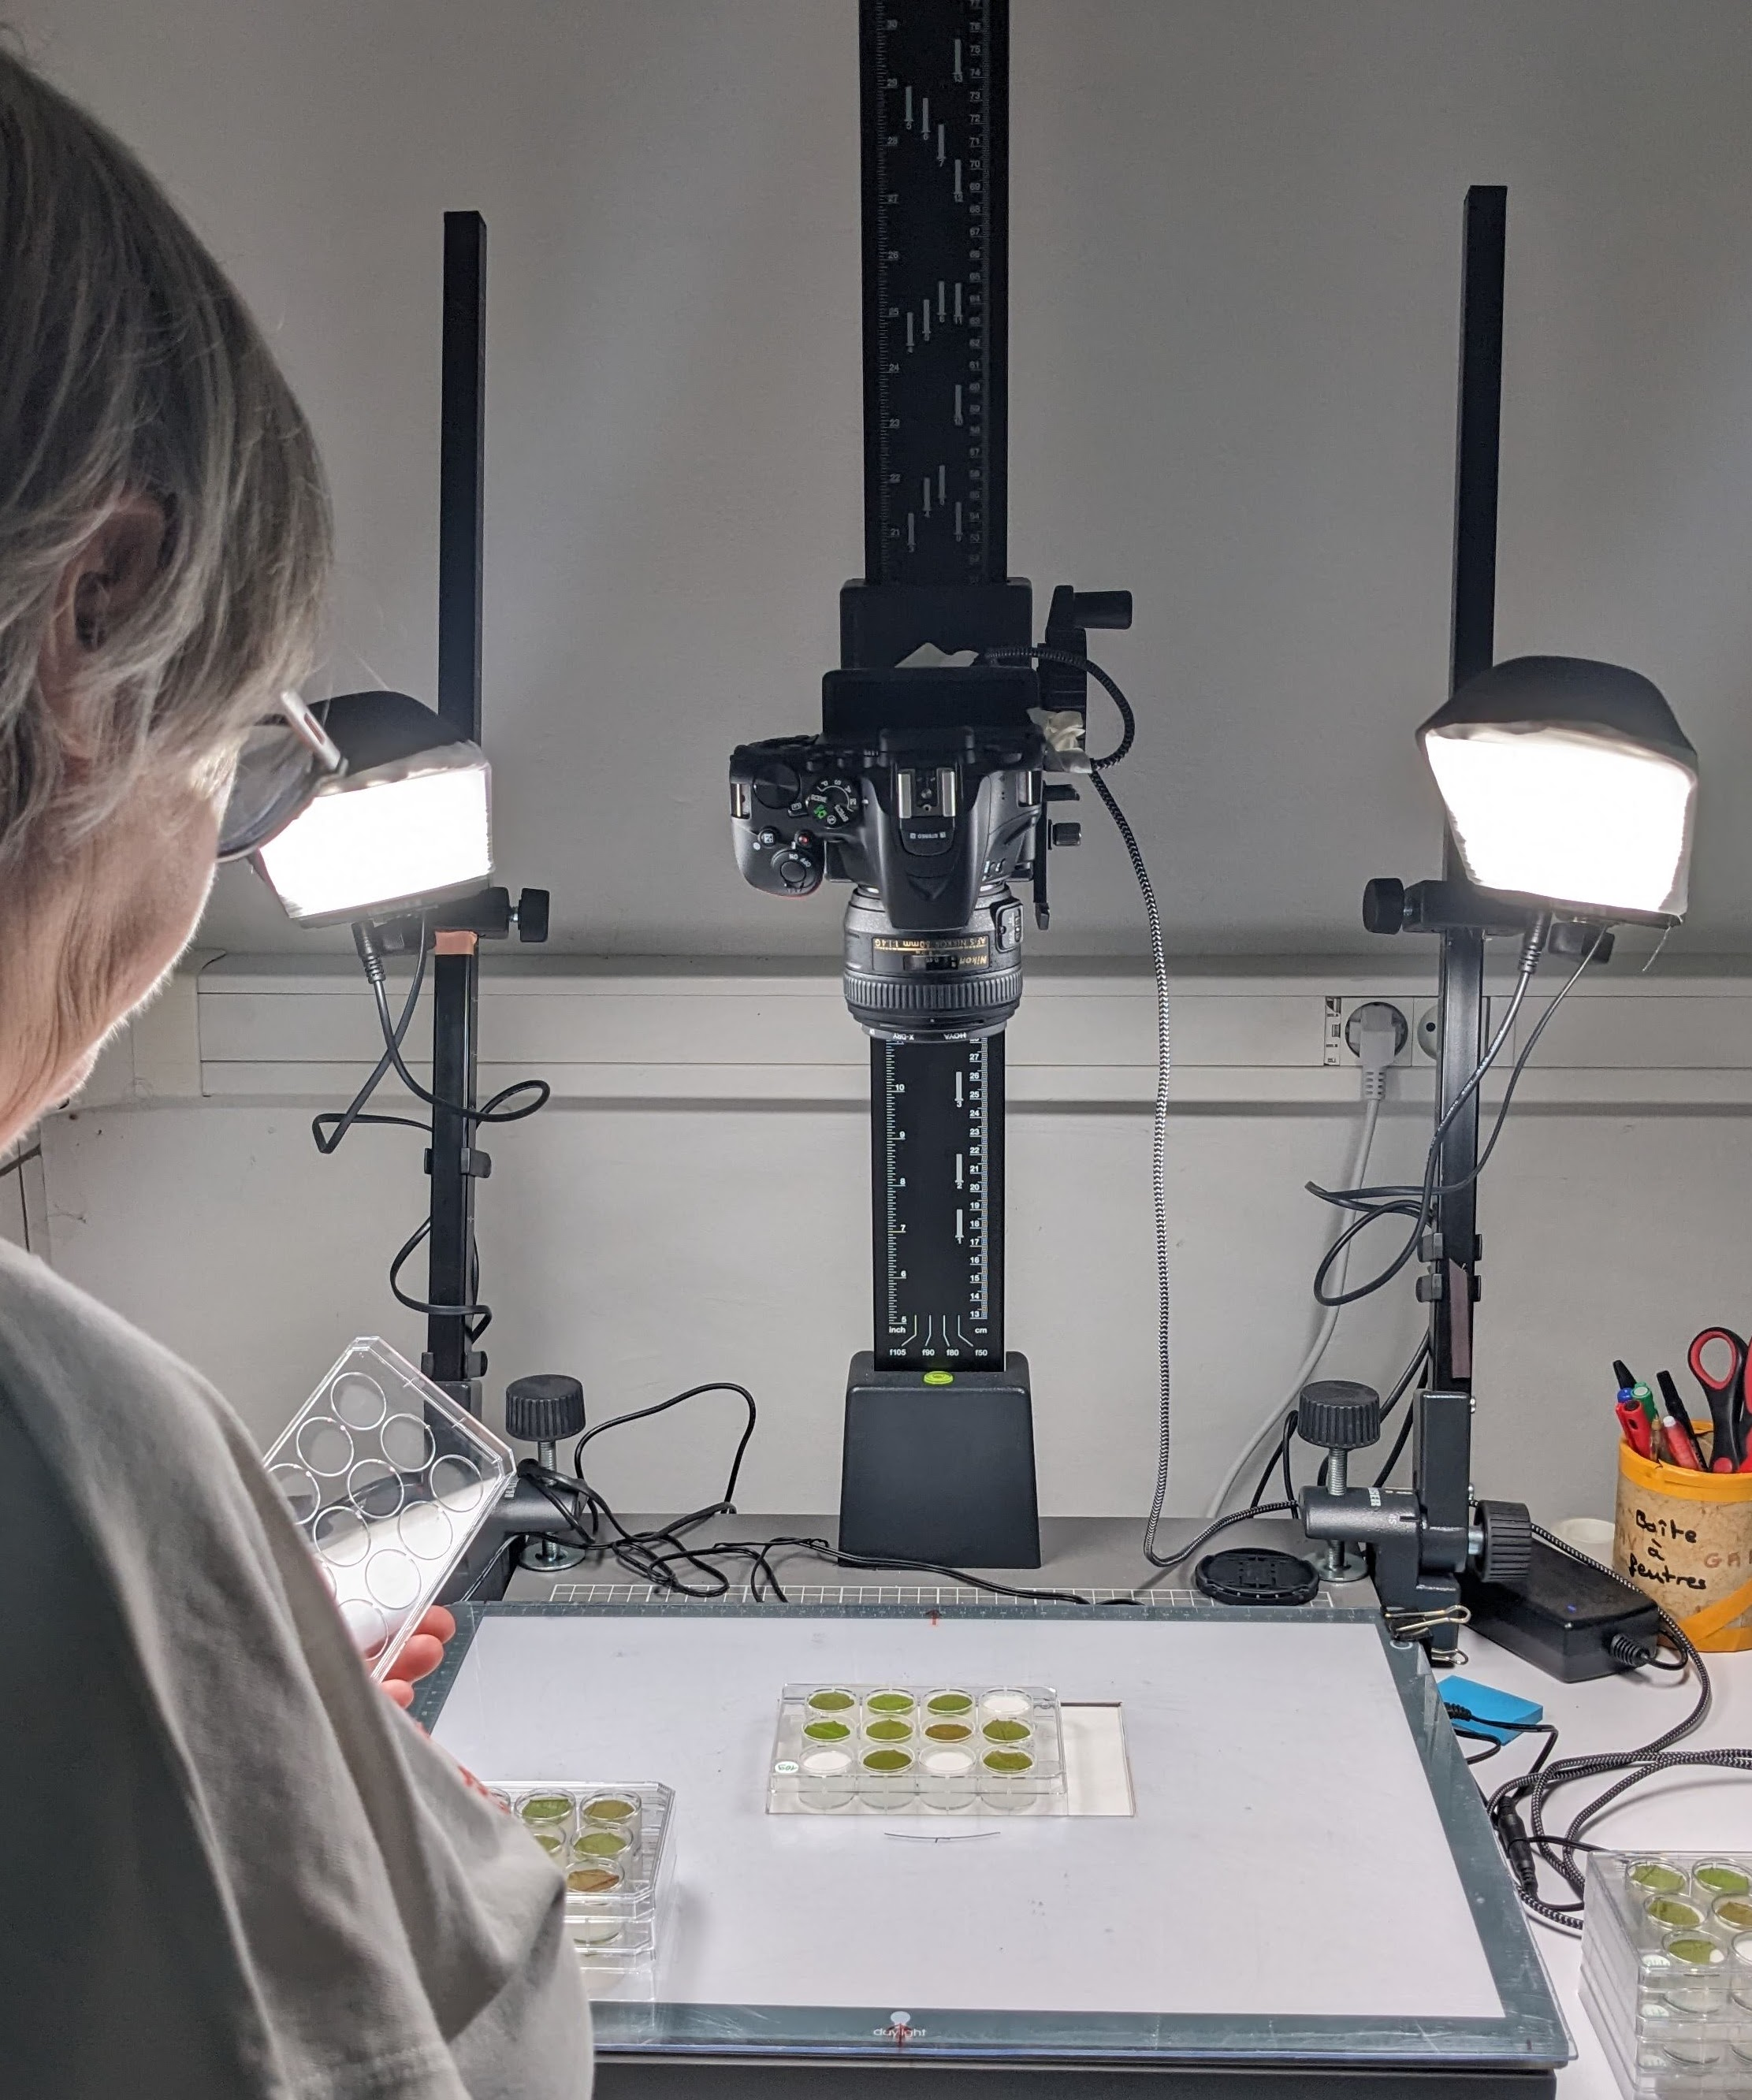
\includegraphics[width=0.5\linewidth]{2023_a_oiv_imaging_system.jpg}
        \caption{VEGOIA platform's manual imaging system}\label{fig:vegoia}
    \end{center}
\end{figure}

\begin{figure}[H]
    \centering
    \begin{subfigure}[b]{0.3\linewidth}
        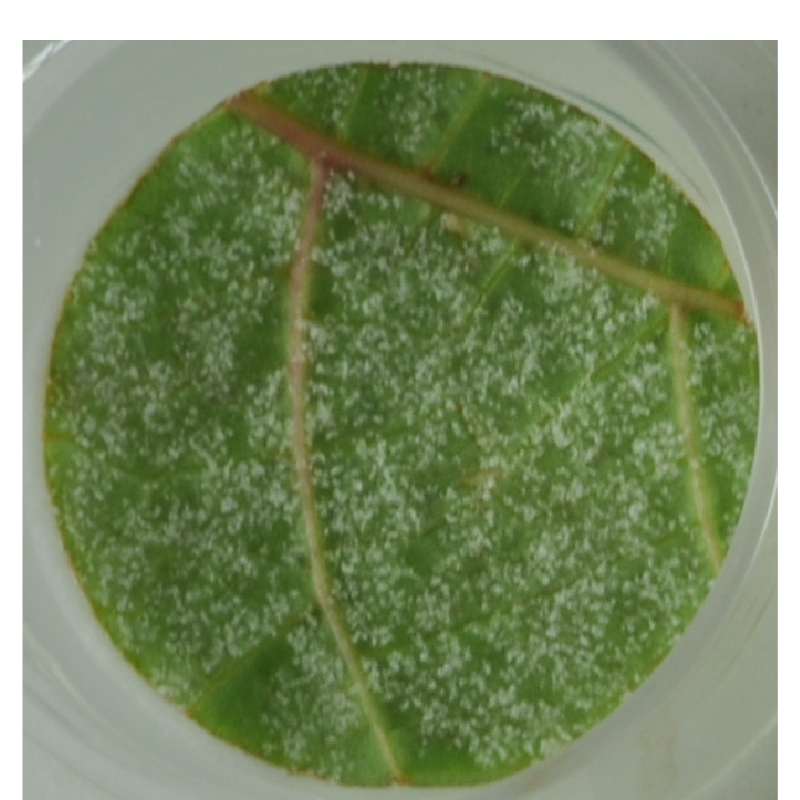
\includegraphics[width=\linewidth]{oiv1.png}
        \caption{OIV 1}\label{fig:oiv1}
    \end{subfigure}
    \begin{subfigure}[b]{0.3\linewidth}
        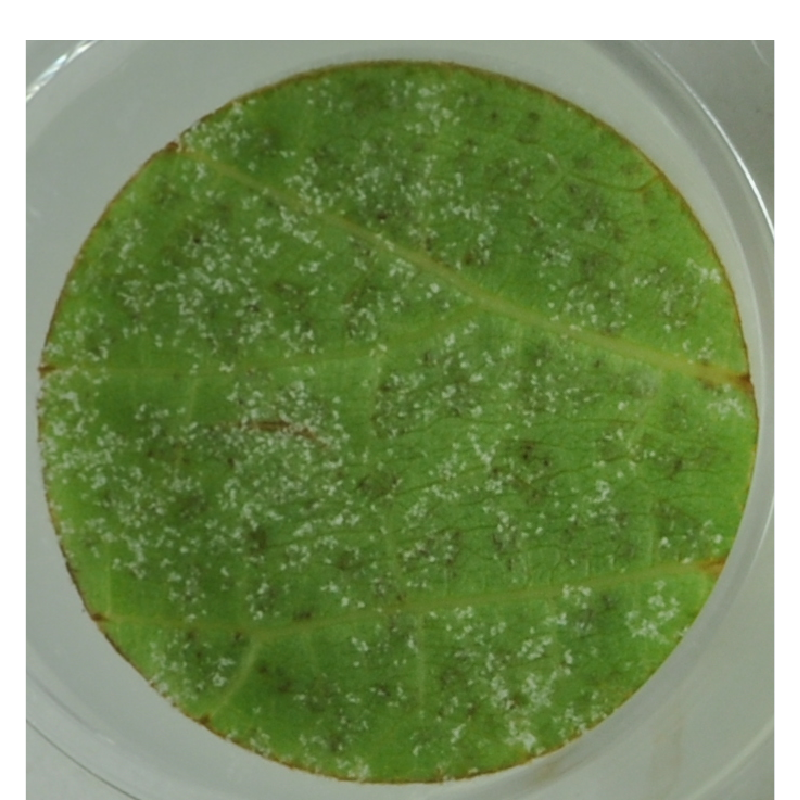
\includegraphics[width=\linewidth]{oiv3.png}
        \caption{OIV 3}\label{fig:oiv3}
    \end{subfigure}
    \begin{subfigure}[b]{0.3\linewidth}
        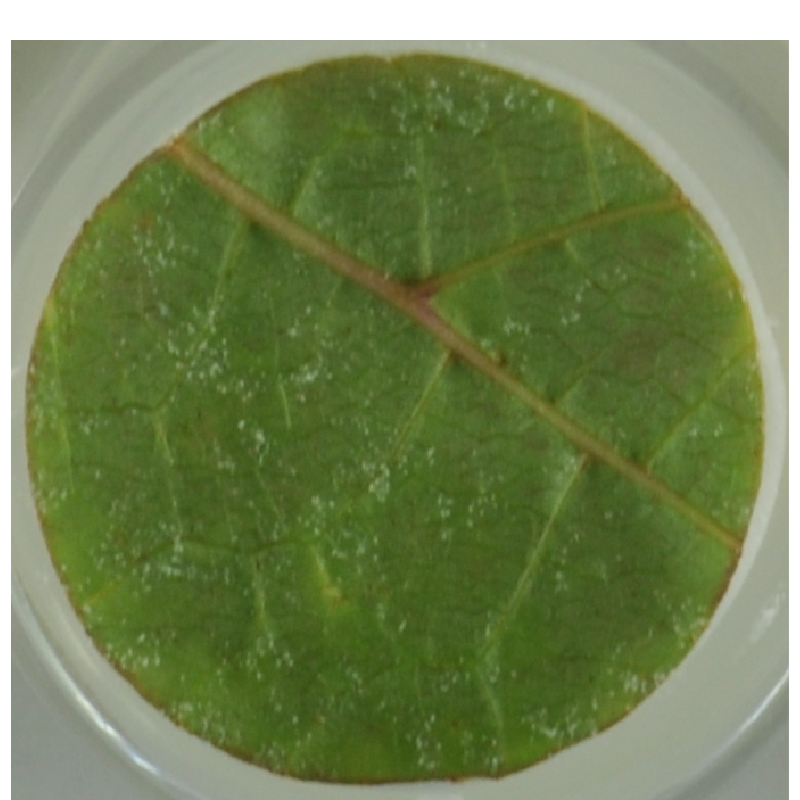
\includegraphics[width=\linewidth]{oiv5.png}
        \caption{OIV 5}\label{fig:oiv5}
    \end{subfigure}
    \begin{subfigure}[b]{0.3\linewidth}
        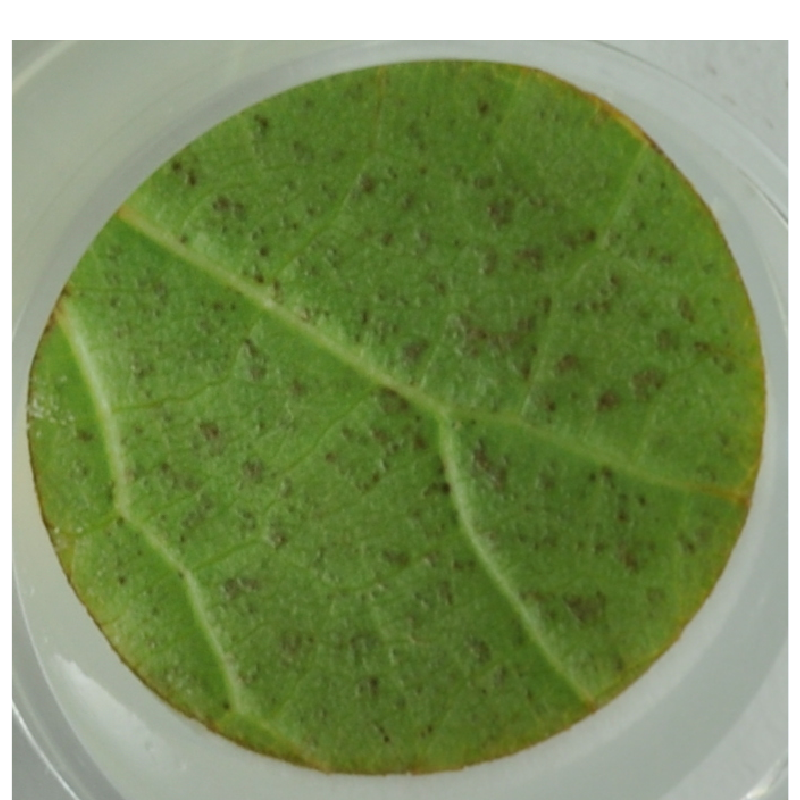
\includegraphics[width=\linewidth]{oiv7.png}
        \caption{OIV 7}\label{fig:oiv7}
    \end{subfigure}
    \begin{subfigure}[b]{0.3\linewidth}
        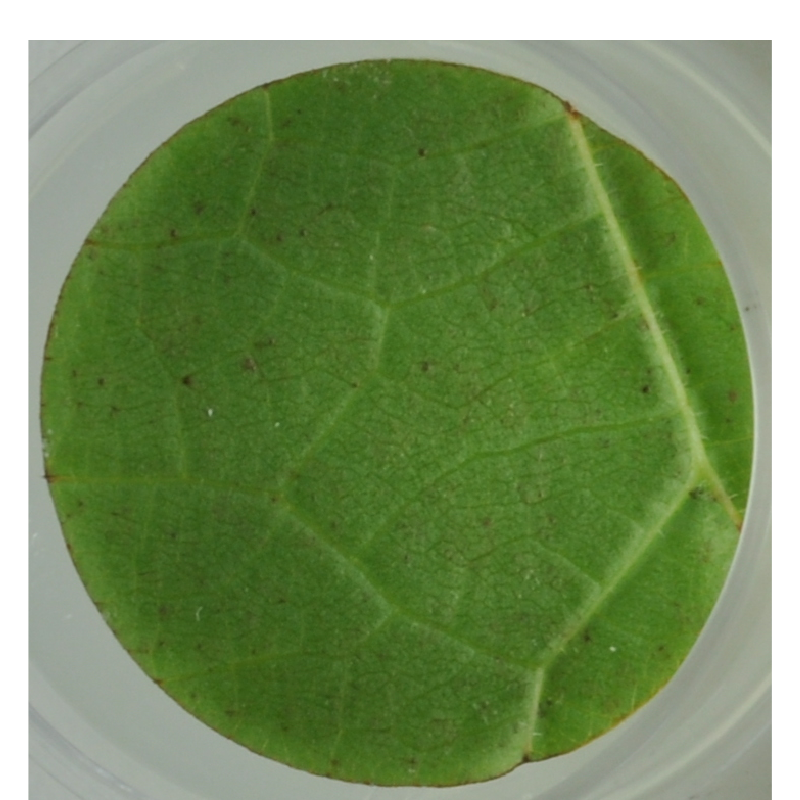
\includegraphics[width=\linewidth]{oiv9.png}
        \caption{OIV 9}\label{fig:oiv9}
    \end{subfigure}
    \caption{Examples of leaf discs annotated with OIV 452-1 values. Levels increase with pathogen resistance. Upper row, susceptible leaf discs with levels 1 to 5. Lower row, resistant leaf disc~\ref{fig:oiv7} and fully resistant leaf disc~\ref{fig:oiv9}}\label{fig:phenotypes}
\end{figure}

\begin{figure}[H]
    \begin{center}
        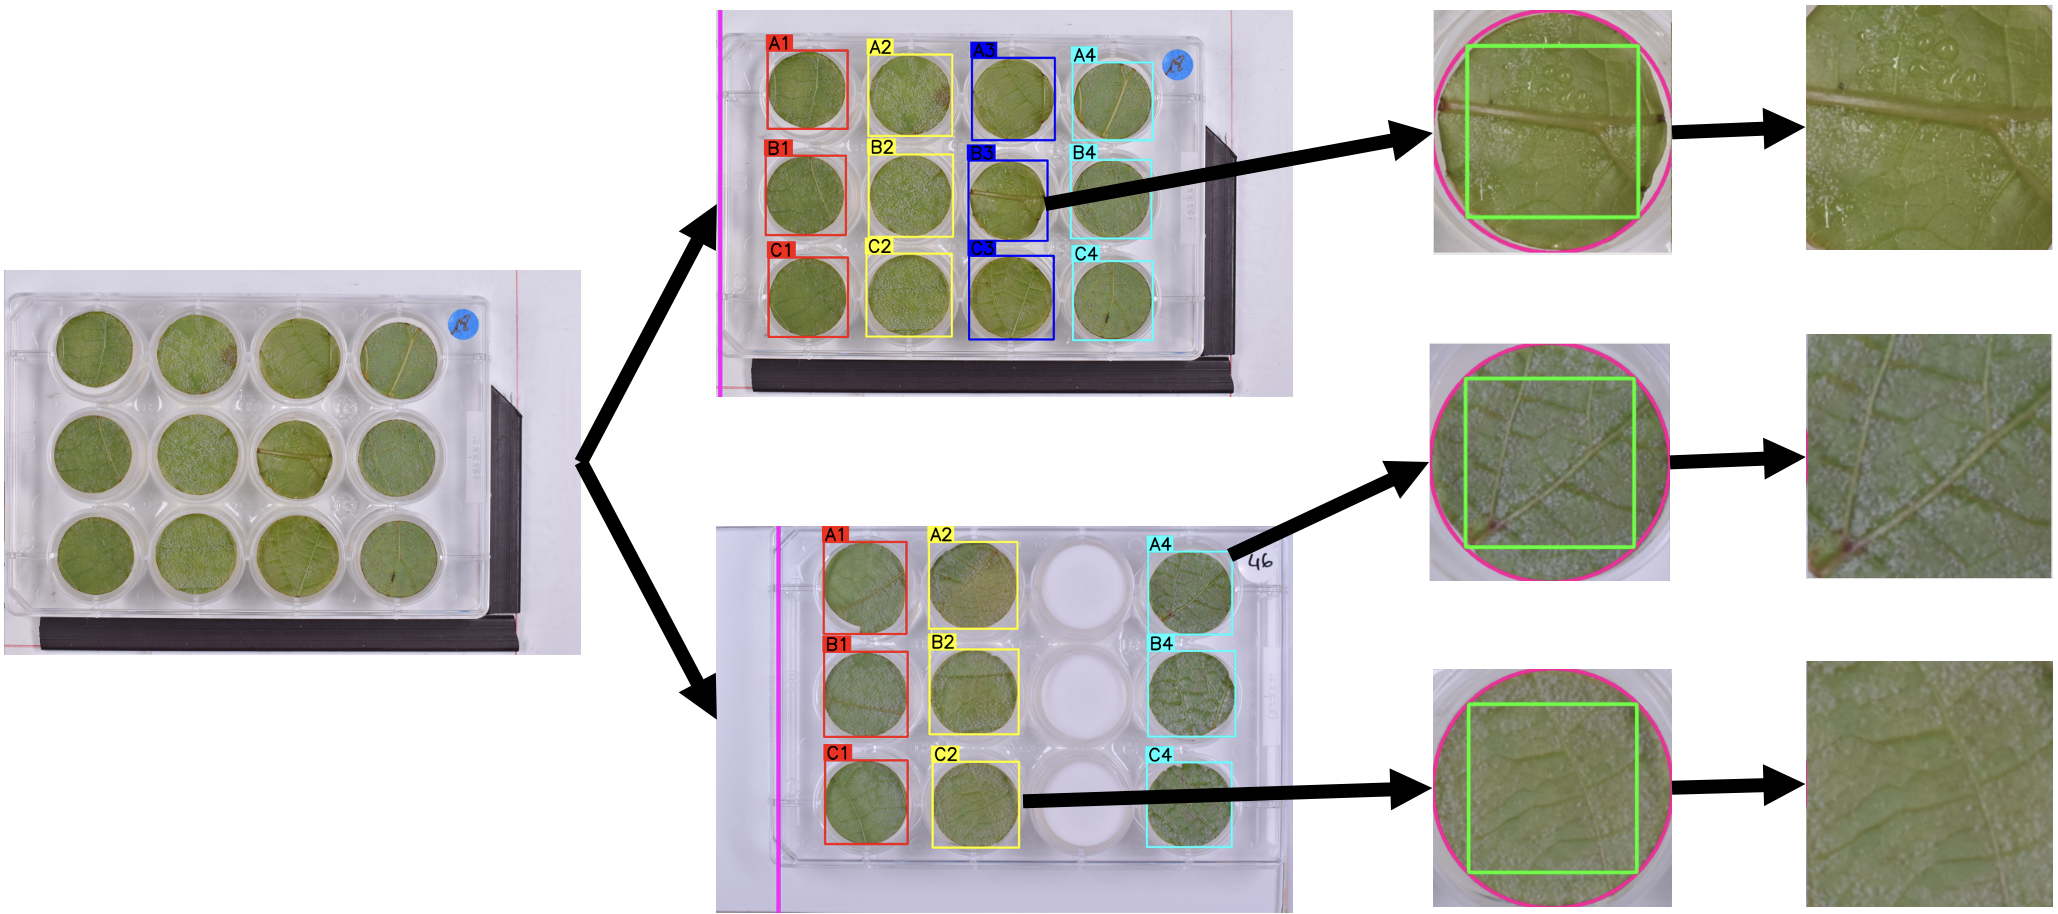
\includegraphics[width=0.9\linewidth]{2023_a_oiv_indexation}
        \caption{Leaf disc extraction workflow}\label{fig:preprocessing}
    \end{center}
\end{figure}

\begin{figure}[H]
    \begin{center}
        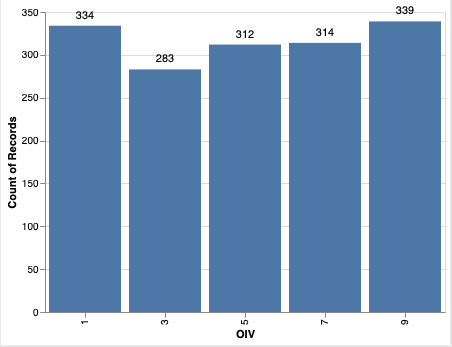
\includegraphics[width=0.7\linewidth]{2023_a_oiv_oiv_distribution}
        \caption{Visualization of the split of the annotated data set for training models}\label{fig:datadistribution}
    \end{center}
\end{figure}

\begin{figure}[H]
    \centering
    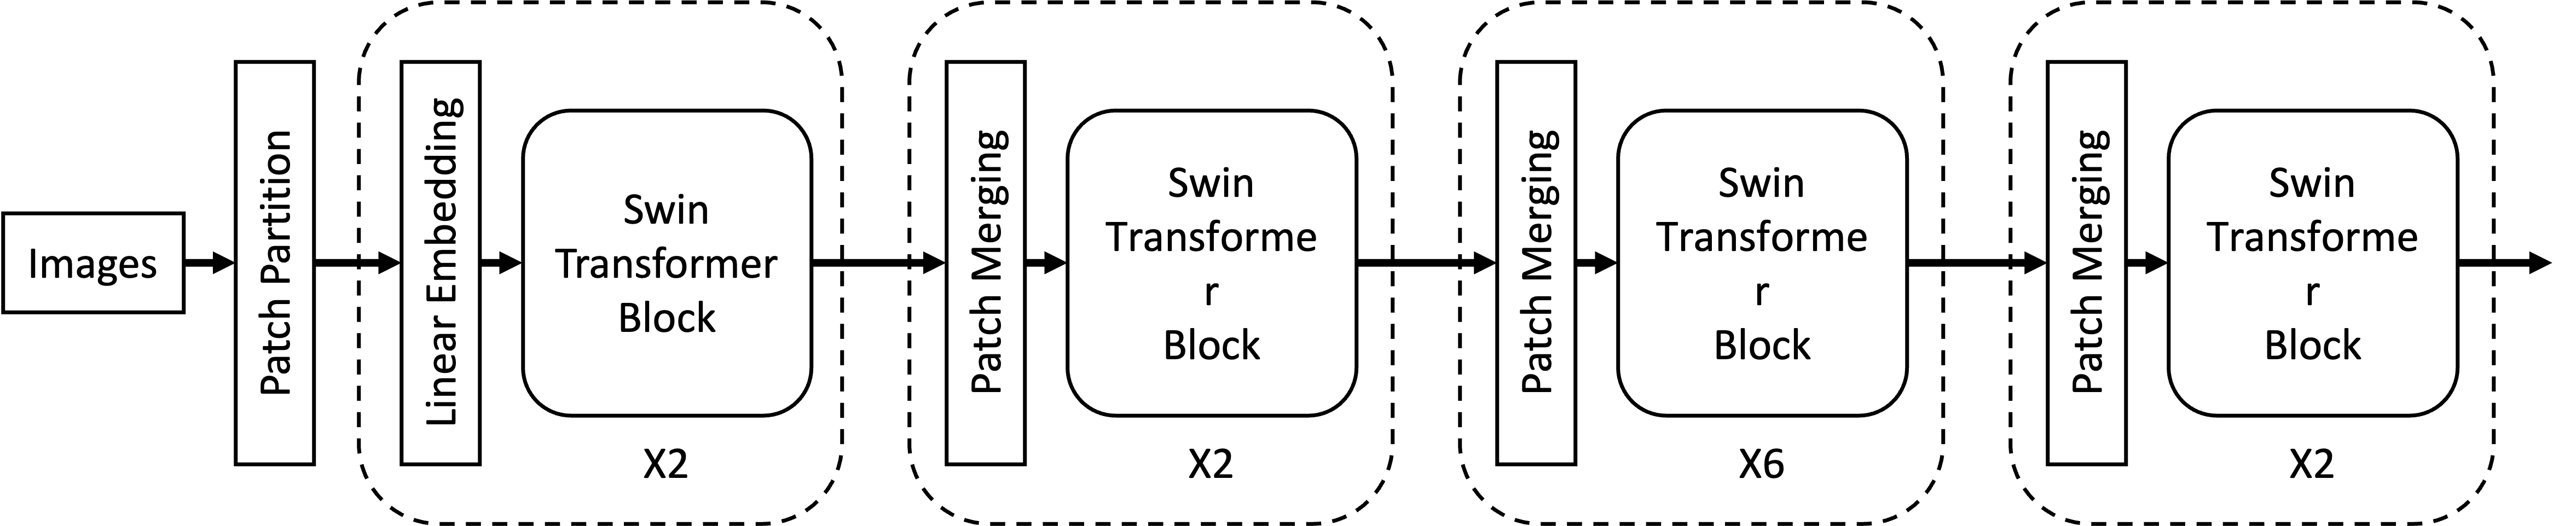
\includegraphics[width=0.9\linewidth]{p_viticola/resources/images/swin_transformer.png}
    \caption{Swin Transformer architecture to serve as backbone for the ordinal regression methods to quantify the symptoms in leaf discs}
    \label{fig:enter-label}
\end{figure}

\begin{equation}
    -\sum_{c=1}^My_{o,c}\log(p_{o,c})\label{fml:crossentropy}
\end{equation}

\begin{equation}
    f(x^{[i]}) = \hat{P}(y^{[i]} > r_{k}|y^{[i]} > r_{k-1})\label{fml:binclass}
\end{equation}

\begin{equation}
    \hat{P}(y^{[i]} > r_{k}) = \prod_{j=1}^{k}f_{j}(x^{[i]})\label{fml:unconditionalprob}
\end{equation}

\begin{equation}
    q^{[i]} = 1 + \sum_{j=1}^{K-1}\mathbb{1}(\hat{P}(y^{[i]} > r_{j}) > 0.5)\label{fml:rankprob}
\end{equation}

\begin{itemize}
    \item Cross entropy loss~\ref{fml:crossentropy}
    \item Binary classification conditional probability~\ref{fml:binclass}
    \item Unconditional probabilities~\ref{fml:unconditionalprob}
    \item Rank prediction~\ref{fml:rankprob}
\end{itemize}

% \begin{equation}
%     \hat{P}(y^{|i|} > r_{1}) \geq \hat{P}(y^{|i|} > r_{2}) \geq ... \geq \hat{P}(y^{|i|} > r_{K-1})\label{fml:}
% \end{equation}


\section{Results and Discussion}


\begin{table}[H]
    \centering
    \caption{Average performance metrics with different ordinal regression modes}
    \label{tab:dtafracevol}
    \begin{tabular}{llrrrr}
        \toprule
        Ordinal regression & backbone   & accuracy & f1 weighted avg & MSE & MAE                                 \\
        \midrule
        Naive              & pretrained & 0.775±0.016                               & 0.769±0.021                   & 0.229±0.018 & 0.227±0.016 \\
        CORAL              & pretrained & 0.447±0.027                               & 0.368±0.055                   & 0.737±0.052 & 0.612±0.024 \\
        CORN               & pretrained & 0.778±0.014                               & 0.772±0.017                   & 0.224±0.015 & 0.223±0.014 \\
        \bottomrule
    \end{tabular}
\end{table}


\begin{table}[H]
\centering
\caption{Confusion matrix precision recall and F1-score where the best ordinal regression method is used, the CORN approach is used}
\label{tab:dtafracevol}
\begin{tabular}{lrrrrrrrr}
\toprule
\textbf{True OIV} & \textbf{Predicted} &&&&  & \textbf{F1-score}\\
{} &   \textbf{1} &   \textbf{3} &   \textbf{5} &   \textbf{7} &   \textbf{9}&&\\
\midrule
\textbf{1} &  41 &   7 &   0 &   0 &   0    & 0.90           \\
\textbf{3} &   2 &  36 &   5 &   0 &   0    & 0.83     \\
\textbf{5} &   0 &   1 &  43 &   3 &   0    & 0.86      \\
\textbf{7} &   0 &   0 &   5 &  69 &  18    & 0.77     \\
\textbf{9} &   0 &   0 &   0 &  15 &  36    & 0.69     \\
\bottomrule
\end{tabular}
\end{table}


% \begin{table}[H]
%     \centering
%     \caption{Classification report}
%     \label{tab:oivcr}
%     \begin{tabular}{lrrrr}
%         \toprule
%         {}           \textbf{precision} & \textbf{recall} & \textbf{f1-score} & \textbf{support} \\
%         \midrule
%         1            & 0.95      & 0.85   & 0.90     & 48      \\
%         3            & 0.82      & 0.84   & 0.83     & 43      \\
%         5            & 0.81      & 0.91   & 0.86     & 47      \\
%         7            & 0.79      & 0.75   & 0.77     & 92      \\
%         9            & 0.67      & 0.71   & 0.69     & 51      \\
%                      &           &        &          &         \\
%         accuracy     &           &        & 0.80     & 281     \\
%         macro avg    & 0.81      & 0.81   & 0.81     & 281     \\
%         weighted avg & 0.80      & 0.80   & 0.80     & 281     \\
%         \bottomrule
%     \end{tabular}
% \end{table}

\section{Conclusions and perspectives}

% \begin{figure}[H]
%     \centering
%     \begin{subfigure}[b]{0.3\linewidth}
%         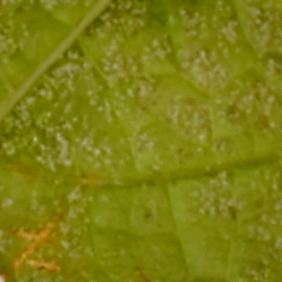
\includegraphics[width=\linewidth]{blur.png}
%         \caption{Blurred image}\label{fig:blurredimage}
%     \end{subfigure}
%     \begin{subfigure}[b]{0.3\linewidth}
%         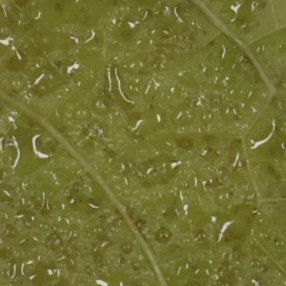
\includegraphics[width=\linewidth]{water.png}
%         \caption{Water droplets}\label{fig:waterimage}
%     \end{subfigure}
%     \begin{subfigure}[b]{0.3\linewidth}
%         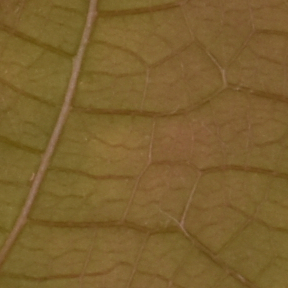
\includegraphics[width=\linewidth]{color.png}
%         \caption{Innate color issue}\label{fig:colorimage}
%     \end{subfigure}
%     \caption{Images with issues are hard to predict by the model}\label{fig:badimages}
% \end{figure}

\begin{figure}[H]
    \centering
    \begin{subfigure}[b]{0.45\linewidth}
        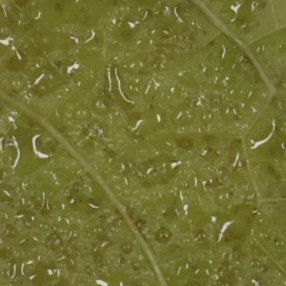
\includegraphics[width=\linewidth]{water.png}
        \caption{Water droplets may be mistaken with sporulation}\label{fig:error97water}
    \end{subfigure}
    \begin{subfigure}[b]{0.45\linewidth}
        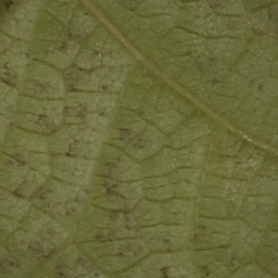
\includegraphics[width=\linewidth]{error_97.png}
        \caption{White stains appear in image}\label{fig:error97b}
    \end{subfigure}
    \caption{Images with OIV value 9 predicted as 7}\label{fig:errors97}
\end{figure}

\begin{figure}[H]
    \centering
    \begin{subfigure}[b]{0.45\linewidth}
        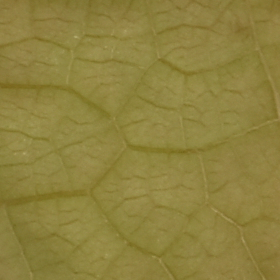
\includegraphics[width=\linewidth]{error_79_2.png}
        \caption{}\label{fig:error79a}
    \end{subfigure}
    \begin{subfigure}[b]{0.45\linewidth}
        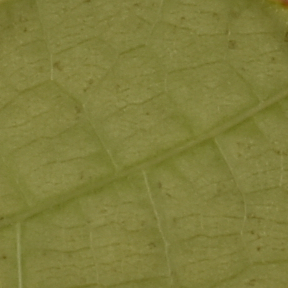
\includegraphics[width=\linewidth]{error_79_1.png}
        \caption{}\label{fig:error79b}
    \end{subfigure}
    \caption{Images with OIV value 7 predicted as 9 when sporulation is hardly perceptible}\label{fig:errors79}
\end{figure}

\textbf{Sabine}
- Améliorer qualité images
    - Eliminer bruit
    - améliorer résolution pour améliorer annotations et modèles
- Prédire QTL
- Entrainer modèle sur images propres
- Tester
    - reste dataset
    - QTLs ?
    - Tester sur pop avec QTLs connus ?
    Tester sur exp qu n'a pas produit des QTLs


\end{document}